\documentclass[12pt,a3paper, landscape]{article}
\usepackage[utf8]{inputenc} 
\usepackage[ngerman]{babel}
\usepackage[T1]{fontenc}
\usepackage{amsmath}
\usepackage{amsfonts}
\usepackage{amssymb}
\usepackage{graphicx}
\usepackage[left=2cm,right=2cm,top=2cm,bottom=2cm]{geometry}
\usepackage{physics}
\usepackage{float}
\usepackage{multirow}
\setlength{\parindent}{0pt}
\usepackage{enumitem}
\usepackage{xcolor}
\usepackage{cancel} 

\newcommand{\h}[2]{\color{#1} #2 \color{black} }

\newcommand{\equalInM}[1]{\h{blue}{#1}} % umfasst mehr; inkl. Vorzeichen gleich über Sym-Anti und Anti-Sym und über die versch. Tableaus dieser Kategorie
\newcommand{\equalInTableau}[1]{\h{magenta}{#1}} % Vorzeichen vertauscht zw. den versch. Tableaus, aber Vorzeichen gleich bzgl. Anti-Sym zu Sym-Anti-Tausch
\newcommand{\equalAntiSym}[1]{\h{brown}{#1}} % zwar nicht in allen Tableaus einer M Sorte, aber gleich (inkl. Vorzeichen) bzgl. der Anti-Sym und der Sym-Anti Rechnung



\usepackage{soul}   % Für das Hervorheben von Text
\usepackage{booktabs}
\usepackage{hhline}
\usepackage{array}
\usepackage{adjustbox}



\begin{document}
\footnotesize

%\begin{adjustbox}{width=\textwidth,totalheight=\textheight,keepaspectratio}


\begin{tabular}{|p{0.5cm}p{1.5cm}
!{\vline width 2pt}p{3cm}!{\vline width 1.25pt}
p{3cm}|p{3cm}|p{3cm}
!{\vline width 1.25pt}p{2cm}p{2cm}|}
\hline 
& & $\left[ 1 ^4\right]$  & 
\multicolumn{3}{c!{\vline width 1.25pt}}{ $\left[ 21 ^2 \right]$}  & \multicolumn{2}{c|}{$\left[ 2^2\right]$}\\
&& 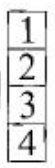
\includegraphics[scale=0.2]{build/young-1hoch4.png} & 
 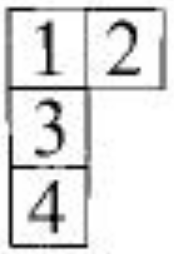
\includegraphics[scale=0.1]{young-21hoch2-12.png}  &  
 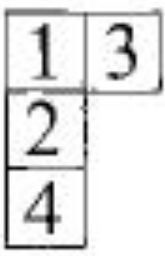
\includegraphics[scale=0.1]{young-21hoch2-13.png} &  
 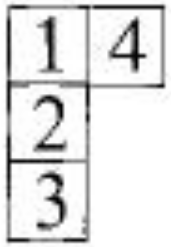
\includegraphics[scale=0.1]{young-21hoch2-14.png} &  
 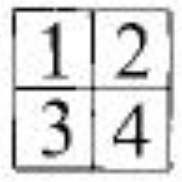
\includegraphics[scale=0.1]{young-2hoch2-12.png} & 
 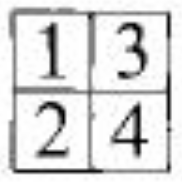
\includegraphics[scale=0.1]{young-2hoch2-13.png}  \\  
 \specialrule{0.2em}{0em}{0em}
$\left[ 1 ^4\right]$  & 
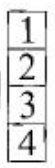
\includegraphics[scale=0.2]{build/young-1hoch4.png} & &  & & &  & 
 \\ \specialrule{0.125em}{0em}{0em}
\multirow{3}{*}{$\left[ 21 ^2 \right]$}	&   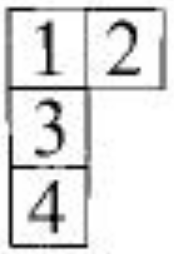
\includegraphics[scale=0.1]{young-21hoch2-12.png}  &  & & &  & & \\
  \cline{2-8} 
 &  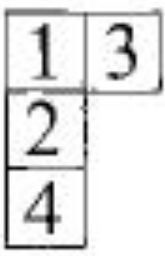
\includegraphics[scale=0.1]{young-21hoch2-13.png}  &  &  & & &  & \\
   \cline{2-8} 
 & 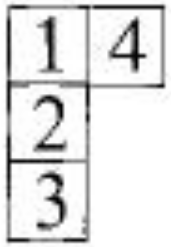
\includegraphics[scale=0.1]{young-21hoch2-14.png}  &  &  & & &  &  \\
 \specialrule{0.125em}{0em}{0em}
\multirow{2}{*}{$\left[ 2^2\right]$} & 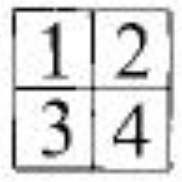
\includegraphics[scale=0.1]{young-2hoch2-12.png} & &  & & &  & \\
& 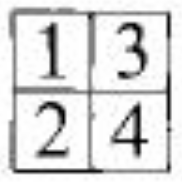
\includegraphics[scale=0.1]{young-2hoch2-13.png}  & &  & & &  & \\  
			\hline 
\end{tabular}\\ \\ 

%\end{adjustbox}

\begin{tabular}{|p{0.5cm}p{1.5cm}
|p{6cm}|
p{3cm}p{3cm}p{3cm}
|p{2cm}p{2cm}|}
\hline 
& & $\left[ 1 ^4\right]$  & 
\multicolumn{3}{c|}{ $\left[ 21 ^2 \right]$}  & \multicolumn{2}{c|}{$\left[ 2^2\right]$}\\
&& 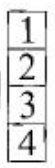
\includegraphics[scale=0.2]{build/young-1hoch4.png} & 
 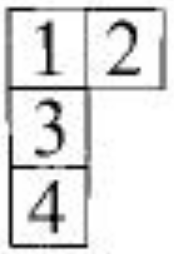
\includegraphics[scale=0.1]{young-21hoch2-12.png}  &  
 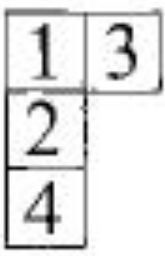
\includegraphics[scale=0.1]{young-21hoch2-13.png} &  
 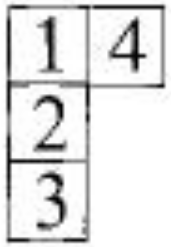
\includegraphics[scale=0.1]{young-21hoch2-14.png} &  
 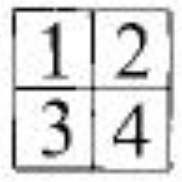
\includegraphics[scale=0.1]{young-2hoch2-12.png} & 
 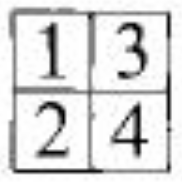
\includegraphics[scale=0.1]{young-2hoch2-13.png}  \\ 
 \hline \rule{0pt}{50pt}
$\left[ 1 ^4\right]$  & 
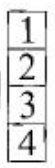
\includegraphics[scale=0.2]{build/young-1hoch4.png} & 
$\left( \begin{array}{c}
+abcd - abdc - acbd + adbc \\
+ acdb - adcb -bacd + badc \\
+ cabd - dabc - cadb + dacb\\
+bcad - bdac - cbad + dbac \\
+ cdab - dcab -bcda + bdca \\
+ cbda - dbca - cdba + dcba 
\end{array}\right)^2$ &  & & &  & 
 \\ \hline 
\multirow{3}{*}{$\left[ 21 ^2 \right]$}	&  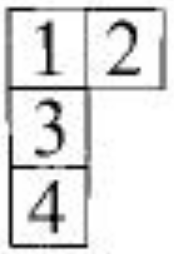
\includegraphics[scale=0.1]{young-21hoch2-12.png}  &  & & &  & & \\ 
 &  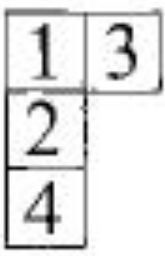
\includegraphics[scale=0.1]{young-21hoch2-13.png}  &  &  & & &  & \\
 & 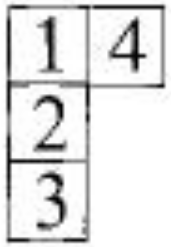
\includegraphics[scale=0.1]{young-21hoch2-14.png}  &  &  & & &  &  \\
 \hline
\multirow{2}{*}{$\left[ 2^2\right]$} & 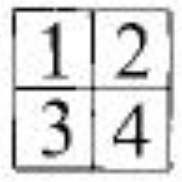
\includegraphics[scale=0.1]{young-2hoch2-12.png} & &  & & &  & \\
& 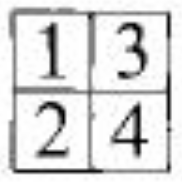
\includegraphics[scale=0.1]{young-2hoch2-13.png}  & &  & & &  & \\  
			\hline 
\end{tabular}\\
   
   
   
   
   
   
   
   
   
   
\end{document}